%!TEX TS-program = xelatex
\documentclass[]{friggeri-cv}
\usepackage{afterpage}
\usepackage{hyperref}
\usepackage{ucs}
\usepackage[utf8x]{inputenc}
\usepackage{color}
\usepackage{xcolor}
\hypersetup{
    pdftitle={Colin LEVERGER},
    pdfauthor={Colin LEVERGER},
    pdfsubject={CV},
    pdfkeywords={CV, Colin LEVERGER, young Data \& DevOps Engineer},
    colorlinks=false,       % no lik border color
    allbordercolors=white    % white border color for all
}
% \addbibresource{bibliography.bib}
\RequirePackage{xcolor}
\definecolor{pblue}{HTML}{4CAF50}

\begin{document}
\header{Colin}{LEVERGER - Ph. D.}
      {Data Engineer \& DevOps - GCP Cloud Architect Certified}

% Fake text to add separator      
\fcolorbox{white}{gray}{\parbox{\dimexpr\textwidth-2\fboxsep-2\fboxrule}{%
.....
}}

% In the aside, each new line forces a line break
\begin{aside}
  
\includegraphics[scale=0.01]{img/white.png}
  \section{Address}
  Centre ville
  35000 RENNES 
  FRANCE
  ~
  \section{Tel}
    +33 (0)6 30 83 62 59 
    ~
  \section{E-Mail}
    \href{mailto:colin.leverger@orange.fr}{\textbf{colin.leverger@}\\orange.fr}
  \section{Web \& Git}
    \href{http://www.colinleverger.fr}{colinleverger.fr}
    \href{https://www.linkedin.com/in/colinleverger}{lnkdin.me/cleverger}
    \href{https://github.com/ColinLeverger}{github/ColinLeverger}
    ~
    \section{Lang. \& Tech.}
    \textbf{Main}:
    \emph{Python}: 5+ years
    \emph{Bash/Unix}: 7+ years
    \textbf{Experienced}:
    \emph{Scala/Java}: 4 years
    \emph{HTML/PHP}: 4 years
    \emph{R}: 3 years
    \textbf{Used in the past}:
    \emph{JavaScript}: 2 years
    \emph{SQL}: 1 year
  %\textbf{Interests \& curiosity}
  %\emph{R}: few projects
    ~
  \section{Spoken}
  \textbf{French}: native
  \textbf{English}: C1+
   ~
   \section{DevOps exp.}
   \emph{Docker}: 5+ years
   \emph{Outils CI}: 4+ years
   \emph{GCP/k8s}: 2+ years
   \emph{Ansible}: 1 year
   \emph{OpenStack}: 1 year
   \emph{ELK}: 1 year
  %\emph{JMeter}: 1 year
    ~
  \section{Interests}
  Data Science, 
  Cybersecurity, 
  Continuous Integration,
  Big Data, etc...
  ~
  \section{Soft skills}
  Autonomy
  Passion
  Curiosity
  Method
  Communication 
  Creativity
  Tenacity
  %\hspace*{-1.3in}
  %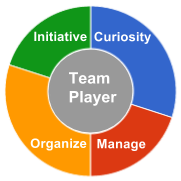
\includegraphics[scale=0.55]{img/personal.png}
    ~
\end{aside}

\section{Experience}
\begin{entrylist}
  \entry
    {01/21 - Now}
    {Data Engineer}
    {\href{http://www.orange.com/en/home}{Orange Innovation}, Rennes - FRANCE}
    {Work in a team of experienced developers on Data Engineering tasks. 
    Development of Cloud solutions (GCP) in Python to facilitate the work of the teams (Data Scientists \& developers).
    Various topics covered (cybersecurity \& CyberHunter, tooling, project management, communication with providers, research in Data Science, etc.). 
    Supervision of an engineering intern. Involvement in the life of the team (on-site ambassador, among others).  
    }
  \entry
    {10/17 - 11/20}
    {Ph.D. candidate}
    {\href{http://www.orange.com/en/home}{Orange Innovation}, Rennes - FRANCE}
    {Research in the field of Capacity Planning. 
    Development of Machine Learning algorithms using Pandas, Python, R, and mining of time series datasets to make predictions in the context of infrastructure performances. 
    Work both at INRIA and Orange Labs. 
    Published 3 papers in national and international conferences (details and references available upon request).
    }
    \vspace{-1.1em}
  \entry
    {2017 - 2022}
    {Lab assistant}
    {Université de Rennes 1 and E.N.S.A.I, Rennes - FRANCE}
    {125 h as a lab assistant at Université de Rennes 1 and E.N.S.A.I Rennes for license and master students. 
    Proposed one CLI application/web scraper in Python 3 as project subject.
    }
    \entry
    {02/19 - 05/19}
    {Visiting researcher}
    {National Institute of Technology, Tokyo - JAPAN}
    {3 months research experience in NII labs at Tokyo. 
    %Work with Ryota KOBAYASHI in the field of time series and study of their seasonality.
    Developed a R Shiny dashboard for displaying massive amount of time series.
    Initiate brand new research collaboration. 
    %Laureate of two mobility grants: 'NII International Internship Program' and 'Bourse de mobilit\'e internationale 2019 - R\'egion Bretagne'.
    }
  \entry
    {09/14 - 09/17}
    {Apprentice Software Engineer}
    {\href{http://www.orange.com/en/home}{Orange Labs \& Services}, Rennes - FRANCE}
    {Apprenticeship to develop software in Scala following a DevOps methodology in a team of 14 Metrology experts. %\underline{Final Project}: dev. of
    % Implemented in bash and Scala a software for infrastructure automatic testing. 
    % Used testing tools such as Gatling and jmeter to stress infrastructure.    
    Experimented with the ELK stack, Grafana and influxdb for massive log processing.
    Developed some Machine Learning algorithms in the Capacity Planning speciality.     
	Use of Scala, Spark, Elasticsearch, Logstash, Kibana, R, Openstack, influxdb, Gatling, Jmeter, etc...
}
  \entry
    {02/15 - Now}
    {Systems and network engineer}
    {On my own, Rennes - FRANCE}
    {Management of my dedicated server. 
    Use of Docker to manage virtual services, Jenkins to do some DevOps and deploy automatically, Ansible to script and configure the server. Play with ELK stack and Grafana dashboards for monitoring the services and cyberattacks.}
%  \entry
%    {04/14 - 07/14}
%    {Internship}
%    {\href{http://www.ait.ie/}{Athlone Institute of Technology}, Athlone - IRELAND}
%    {Three months end-of-course internship; preparation of project subjects for students. Worked with \emph{Arduino}, \emph{Java}, \emph{HTML/CSS}, \emph{PHP} and \emph{C}.}
\end{entrylist}

%\section{Research \& Publications}
%\begin{entrylist}
%  \entry
%    {10/19}
%    {IDEAL Conference (C)}
%    {Manchester - UNITED KINGDOM}
%    {"Toward a framework for seasonal time series forecasting using clustering.", Leverger, C., Malinowski, S., Guyet, T., Lemaire, V., Bondu, A., \& Termier, A.}
%  \entry
%    {09/18}
%    {AALTD workshop at ECML (A)}
%    {Dublin - IRELAND}
%    {"Day-ahead time series forecasting : application to capacity planning.", Leverger, C., Lemaire, V., Malinowski, S., Guyet, T., \& Rozé, L.}
%\end{entrylist}

\section{Higher education}
\begin{entrylist}
  \entry
    {09/16 - 02/17}
    {ERASMUS}
    {\href{http://www.ruc.dk/en/}{Roskilde University}, Roskilde - DENMARK}
    {5 months abroad, ERASMUS exchange in Denmark for the last academic semester of my Master Degree. \underline{Main subjects}: IT-architecture and user driven software design, Security, Big Data, Danish.}
  \entry
    {09/14 - 09/17}
    {Master 2 Degree in Computer Engineering}
    {\href{http://www.enssat.fr}{E.N.S.S.A.T.}, Lannion - FRANCE}
    {Curriculum Networking, Multimedia \& Computing Science. \underline{Main subjects}: Network Applications, Systems Architecture, Design of Services \& of User Interfaces. Participated to a lot of software development projects, some of those can be found in my web portfolio \href{https://colinleverger.fr}{https://colinleverger.fr}}
  %\entry
  %  {2012 - 2014}
  %  {Two year Undergraduate University Degree of Technology in Electronics and Computing}
  %  {\href{https://iut-rennes.univ-rennes1.fr/les-6-departements/genie-electrique-informatique-industrielle}{Universit\'e de Rennes 1}, Rennes - FRANCE}
  %  {Main subjects: Programming, Microchip, Digital and Analogic Electronics.}
% \vspace{-1.2em}  
%   \entry
%     {2016  -  2017}
%     {MOOCs and online courses}
%     {Coursera and edX, e-learning}
%     {Learning Functional paradigm with the Scala language. The course is complemented by a series programming projects as homework assignments. Learning Google Cloud Platform: SDKs \& CLI, VMs management, Scalability, ...}
\end{entrylist}

%\section{Certifications}
%\begin{entrylist}
%  \entry
%    {07/16 - 02/17}
%    {Scala Specialization}
%    {Coursera, E-learning}
%    {Learning Functional paradigm with the Scala language. The course is complemented by a series programming projects as homework assignments.}
  %\entry
  %  {01/17 - 02/17}
  %  {Google Cloud Platform Specialization}
  %  {Coursera, E-learning}
  %  {Learning Google Cloud Platform: SDKs \& CLI, VMs management, Scalability, ...}
%\end{entrylist}

\section{Skills}
\begin{entrylist}
%  \entry
%    {Computing}
%    {Languages}
%    {}
%    {Python, R, Scala, Java, C, HTML/CSS, PHP, JavaScript, Bash/scripting, SQL, NoSQL, \LaTeX}
  \entry
%    {}
    {Computing}
%    {Paradigms}
%    {}
%    {Functional, imperative, object-oriented, concurrent programming, real-time programming}
%  \entry
%    {}
    {Notable tools}
    {}
    {FastAPI, Gitlab-CI, Pandas, NumPy, scikit-learn, Tensorflow, Matplotlib, Jupyter Notebook, R, ggplot2, Git, Spark, influxDB, massive grid computing, Khiops coclustering tool @Orange}
  % \entry
  %   {Hobbies}
  %   {Music}
  %   {}
  %   {Creation and composition, beatmaking, recording and sound engineering for my own band. We interpret only our original creations, that are available online on streaming services. Intensive use of Ableton 10 and of machines, both for music production and live performances.}
  \entry
  {}
  {MOOCs Coursera \& Certifications}
  {}
  {GCP Cloud Architect Certification 2023, Scala Specialization, Data Engineering GCP, etc.}
  \entry
    {Hobbies}
    {Sport}
    {}
    {Ashtanga Yoga, intermediate level. Regular runner, climber and swimmer.}
\end{entrylist}
\end{document}